\chapter{原型系统设计与实现}

    原型系统包括核心工具Lapis和用户接口两大组件. 其中, 核心工具提供从脚本解析到测试生成与执行的整套方法的原型实现. 用户接口则包括核心工具的编程API接口, 和在线API脚本的上传、编辑和可视化的web应用. 以上各部分完全独立.

    % extended version
    % 原型系统包括核心工具Lapis和用户接口两大组件. 其中, 核心工具提供从脚本解析到测试生成与执行的整套方法的原型实现. 用户接口则包括核心工具的编程API接口, 和在线API脚本的上传、编辑和可视化的web应用, 以及桌面端测试管理系统. 以上各部分完全独立.

	\section{核心工具Lapis}
	
	    \begin{figure}[!htb]
	        \centering
	        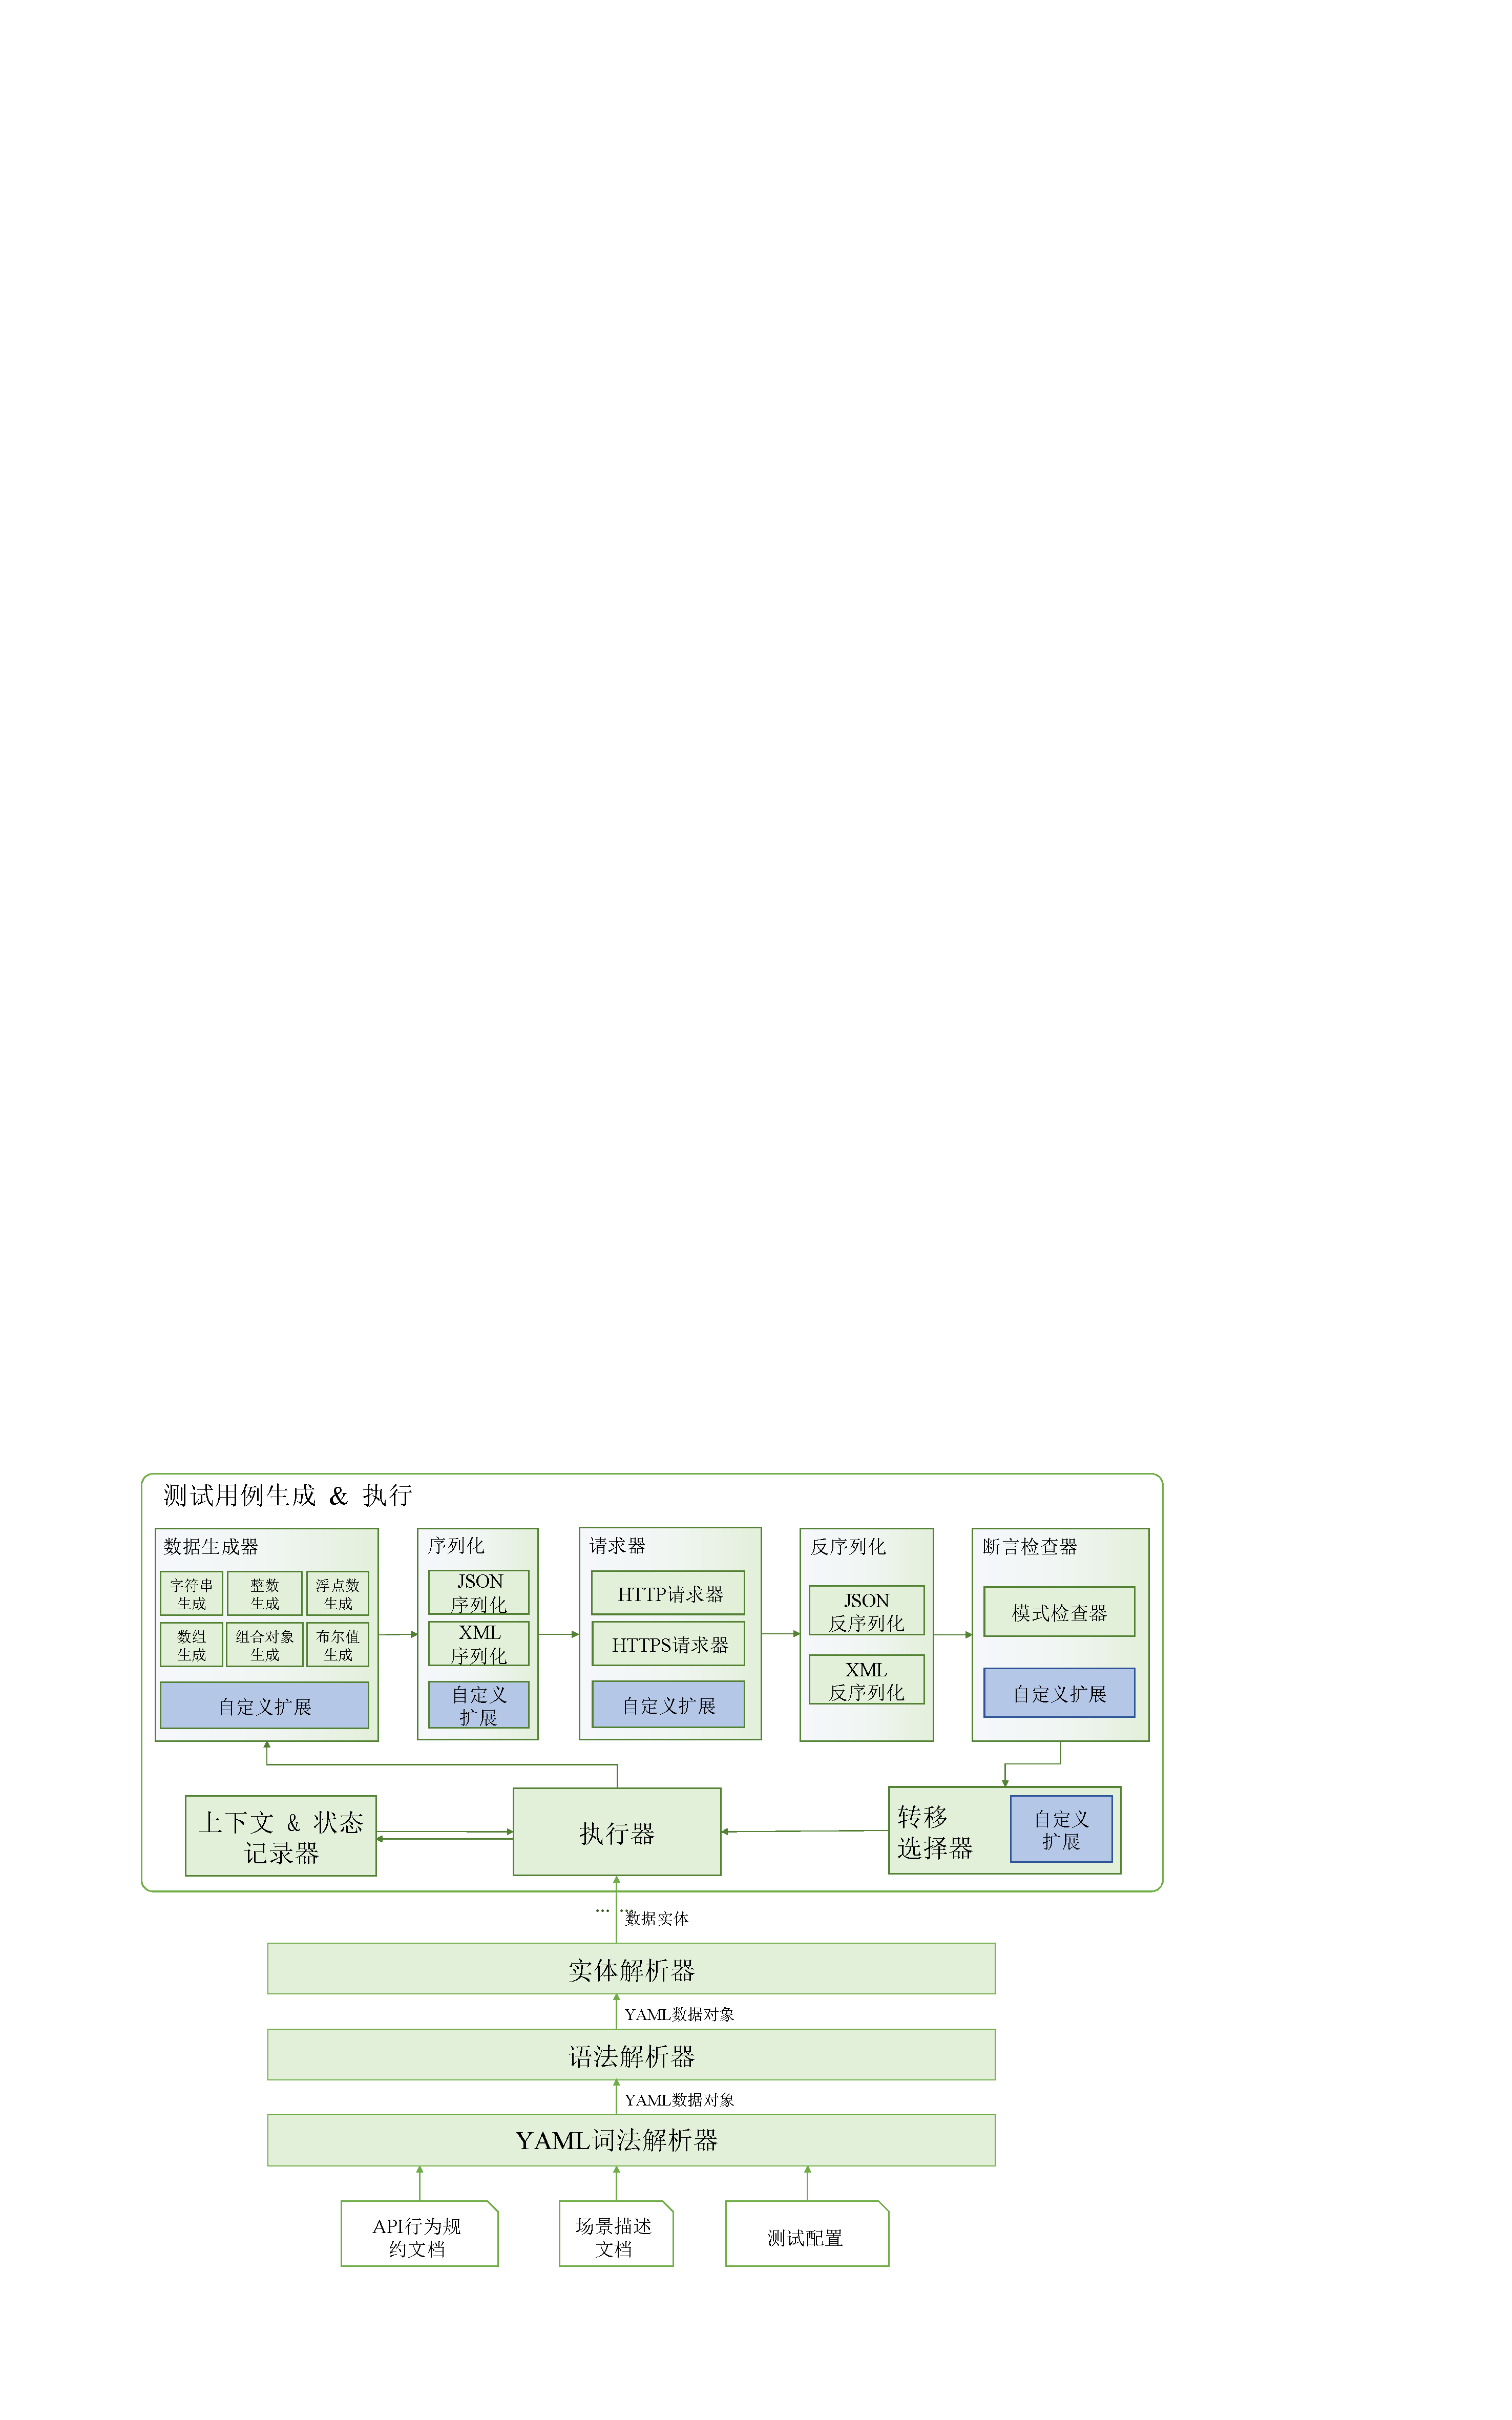
\includegraphics[width=300pt]{tool_architecture3.pdf}
	        \caption{Lapis工具整体架构. 工具的输入为API行为规约文档, 场景描述文档和测试配置. 输出为测试用例及其执行结果. 执行流在图中从下往上, 从左往右.}
	        \label{fig:lapis_arch}
	    \end{figure}
	    
	    图\ref{fig:lapis_arch}展示了Lapis工具原型的整体架构.
	    
	    工具完全采用Python 3实现. 其依赖于一些Python开源库, 如Requests\footnote{http://docs.python-requests.org}, PyYAML\footnote{https://pyyaml.org}, rstr\footnote{https://pypi.org/project/rstr/2.1.1}, 以及标准库.
	    
	    工具的输入为三个脚本文件 - 使用OpenAPI规约语言描述的API行为文档, YAML格式的场景模型文档, 以及YAML格式的测试配置文档. 本工作定义了一套格式规范, 用于表述场景模型. 测试配置文档为可选项, 内容较简单, 对API行为文档进行了一定补充, 并提供定制运行参数的功能. 三个脚本文件具有一定的层次关系: API行为文档提供了API的具体描述, 包括请求数据, 响应数据, 请求方法, 请求URL, 请求协议等; 场景模型文档利用这些信息, 并将场景模型的状态与对应API描述关联起来, 同时为自动化测试提供具体的场景模型; 测试配置文档则提供少量运行所需参数, 并支持一些可定制选项, 如指定测试用例生成与执行的时间限制等.
	    
	    \label{sec:lapis_impl}
	    工具的输出为包含所有测试用例及其执行结果的Python列表, 列表的各个元素即为各个测试用例, 包括测试用例的执行序列, 生成的请求数据, 获得的响应结果, 响应时间及模型覆盖率等信息.

	    工具采用模块化的设计, 具有良好的可扩展性, 如图\ref{fig:lapis_arch}所示, 多个模块均支持用户自定义:
	    \begin{itemize}
	        \item 在场景模型中, 如\ref{sec:set_define}小节所述, 定义合法输入, 合法响应和转移条件可以采用自定义校验函数(对应断言检查器模块和转移选择器模块的用户扩展)和自定义生成函数(对应数据生成器模块的用户扩展);
	        
	        \item 在请求器中, 为了支持各种不同的API服务, 除了已实现的HTTP协议缺省请求器和HTTPS协议缺省请求器外, 用户可以通过子类化抽象接口类的方法编写自定义请求器. 如, 通过这种方式, 对使用签名机制的API使用专用请求器;
	        
	        \item 在序列化模块中, 除了默认的JSON格式和XML格式序列化模块外, 用户也可以用子类化的方法, 实现自定义的序列化格式;
	        
	        \item 在转移选择器模块中, 除了直接按转移概率随机选择转移外, 用户也可以实现接口函数并在测试配置文档中引入, 来应用启发式转移选择算法;
	        
	        \item 此外, 在全局测试配置中, 为了更好地与被测系统(SUT)交互, 工具提供了用于被测系统启动, 停止和请求间隔操作的函数接口, 在测试配置文档中指定函数的所在位置, 即可引入这些自定义交互函数.
	    \end{itemize}  
	    自定义函数和子类的引入得益于Python的动态反射机制, 但这也要求这些自定义扩展使用Python实现.
	    
	    工具各个模块的功能如下:
	    
	    \begin{itemize}
	        \item YAML词法解析器:\\
	            此模块分析输入的三个脚本文件的格式, 检查它们是否为合法YAML文档, 并建立文档树.
	        \item 语法解析器:\\
	            此模块读入数据对象, 检查每个脚本是否包括必需域以及各个域的数据合法性, 比如API行为文档中各个API参数的定义是否合法, 场景模型文档中转移的定义是否合法等.
	        \item 实体解析器:\\
	            此模块从脚本中提取出自动化测试所需信息, 而如开发者联系方式域(\texttt{info.contact}域)等无关域则被舍去. 提取的信息使用数据实体(Python类实例)存储, 并传给测试执行器.
	        \item 测试执行器:\\
	            测试执行器调度和控制整个测试用例的生成和执行过程. 执行器也负责处理用户自定义扩展抛出的异常, 防止系统崩溃. 用户编程接口(见\ref{sec:program_interface}小节)直接与此模块进行交互.
	        \item 上下文\&状态记录器:\\
	            此模块记录测试的所有有价值信息, 最后返回给用户.
	        \item 数据生成器:\\
	            此模块生成请求参数(输入数据).
	        \item 序列化:\\
	            此模块将生成的请求参数序列化/格式化为字符串.
	        \item 请求器:\\
	            此模块发送请求, 并收集响应结果. 负责处理网络交互的细节, 也可以进行自定义扩展使之支持签名机制.
	        \item 反序列化:\\
	            此模块将响应的头和响应体分离, 并根据API行为文档和测试配置文档中的数据格式定义, 将字符串解析为数据实体.
	        \item 断言检查器:\\
	            此模块对响应数据进行检查, 包括模式检查(是否符合定义的模式)和断言检查(是否满足上下文依赖和约束)两个方面.
	        \item 转移选择器:\\
	            此模块随机选择转移边, 确定当前执行序列的下一状态.
	    \end{itemize}

	\section{用户接口}
		\subsection{编程接口}
            \label{sec:program_interface}
            用户可以通过调用编程接口直接使用核心工具Lapis. 编程接口为Python函数的形式, 封装并隐藏了工具实现的具体细节. 普通用户使用\texttt{run()}函数, 即可一行完成测试生成与执行. \texttt{run()}函数的签名如下:
            \begin{flushleft}
                \scriptsize
                \tt
                \begin{lstlisting}[language=python]
def run(api_doc_path, scenario_doc_path, testconf_doc_path=None, num_case=1, verbose=0)
                \end{lstlisting}
            \end{flushleft}
            用户需要提供三个脚本文件的路径(测试配置脚本可选), 生成测试用例的总数, 以及往控制台输出信息的详细级别. 函数的返回值即为工具的输出, 包含内容详见\ref{sec:lapis_impl}小节, 为包含所有测试用例及其执行结果的Python列表.
            
		\subsection{web端脚本编辑系统}

            本文的工具与方法使用结构化的脚本文档作为输入, 脚本文档则常常需要手工编写, 因此, 用户友好的脚本编辑和管理工具不可或缺.
            
            \begin{figure}[!htb]
                \centering
                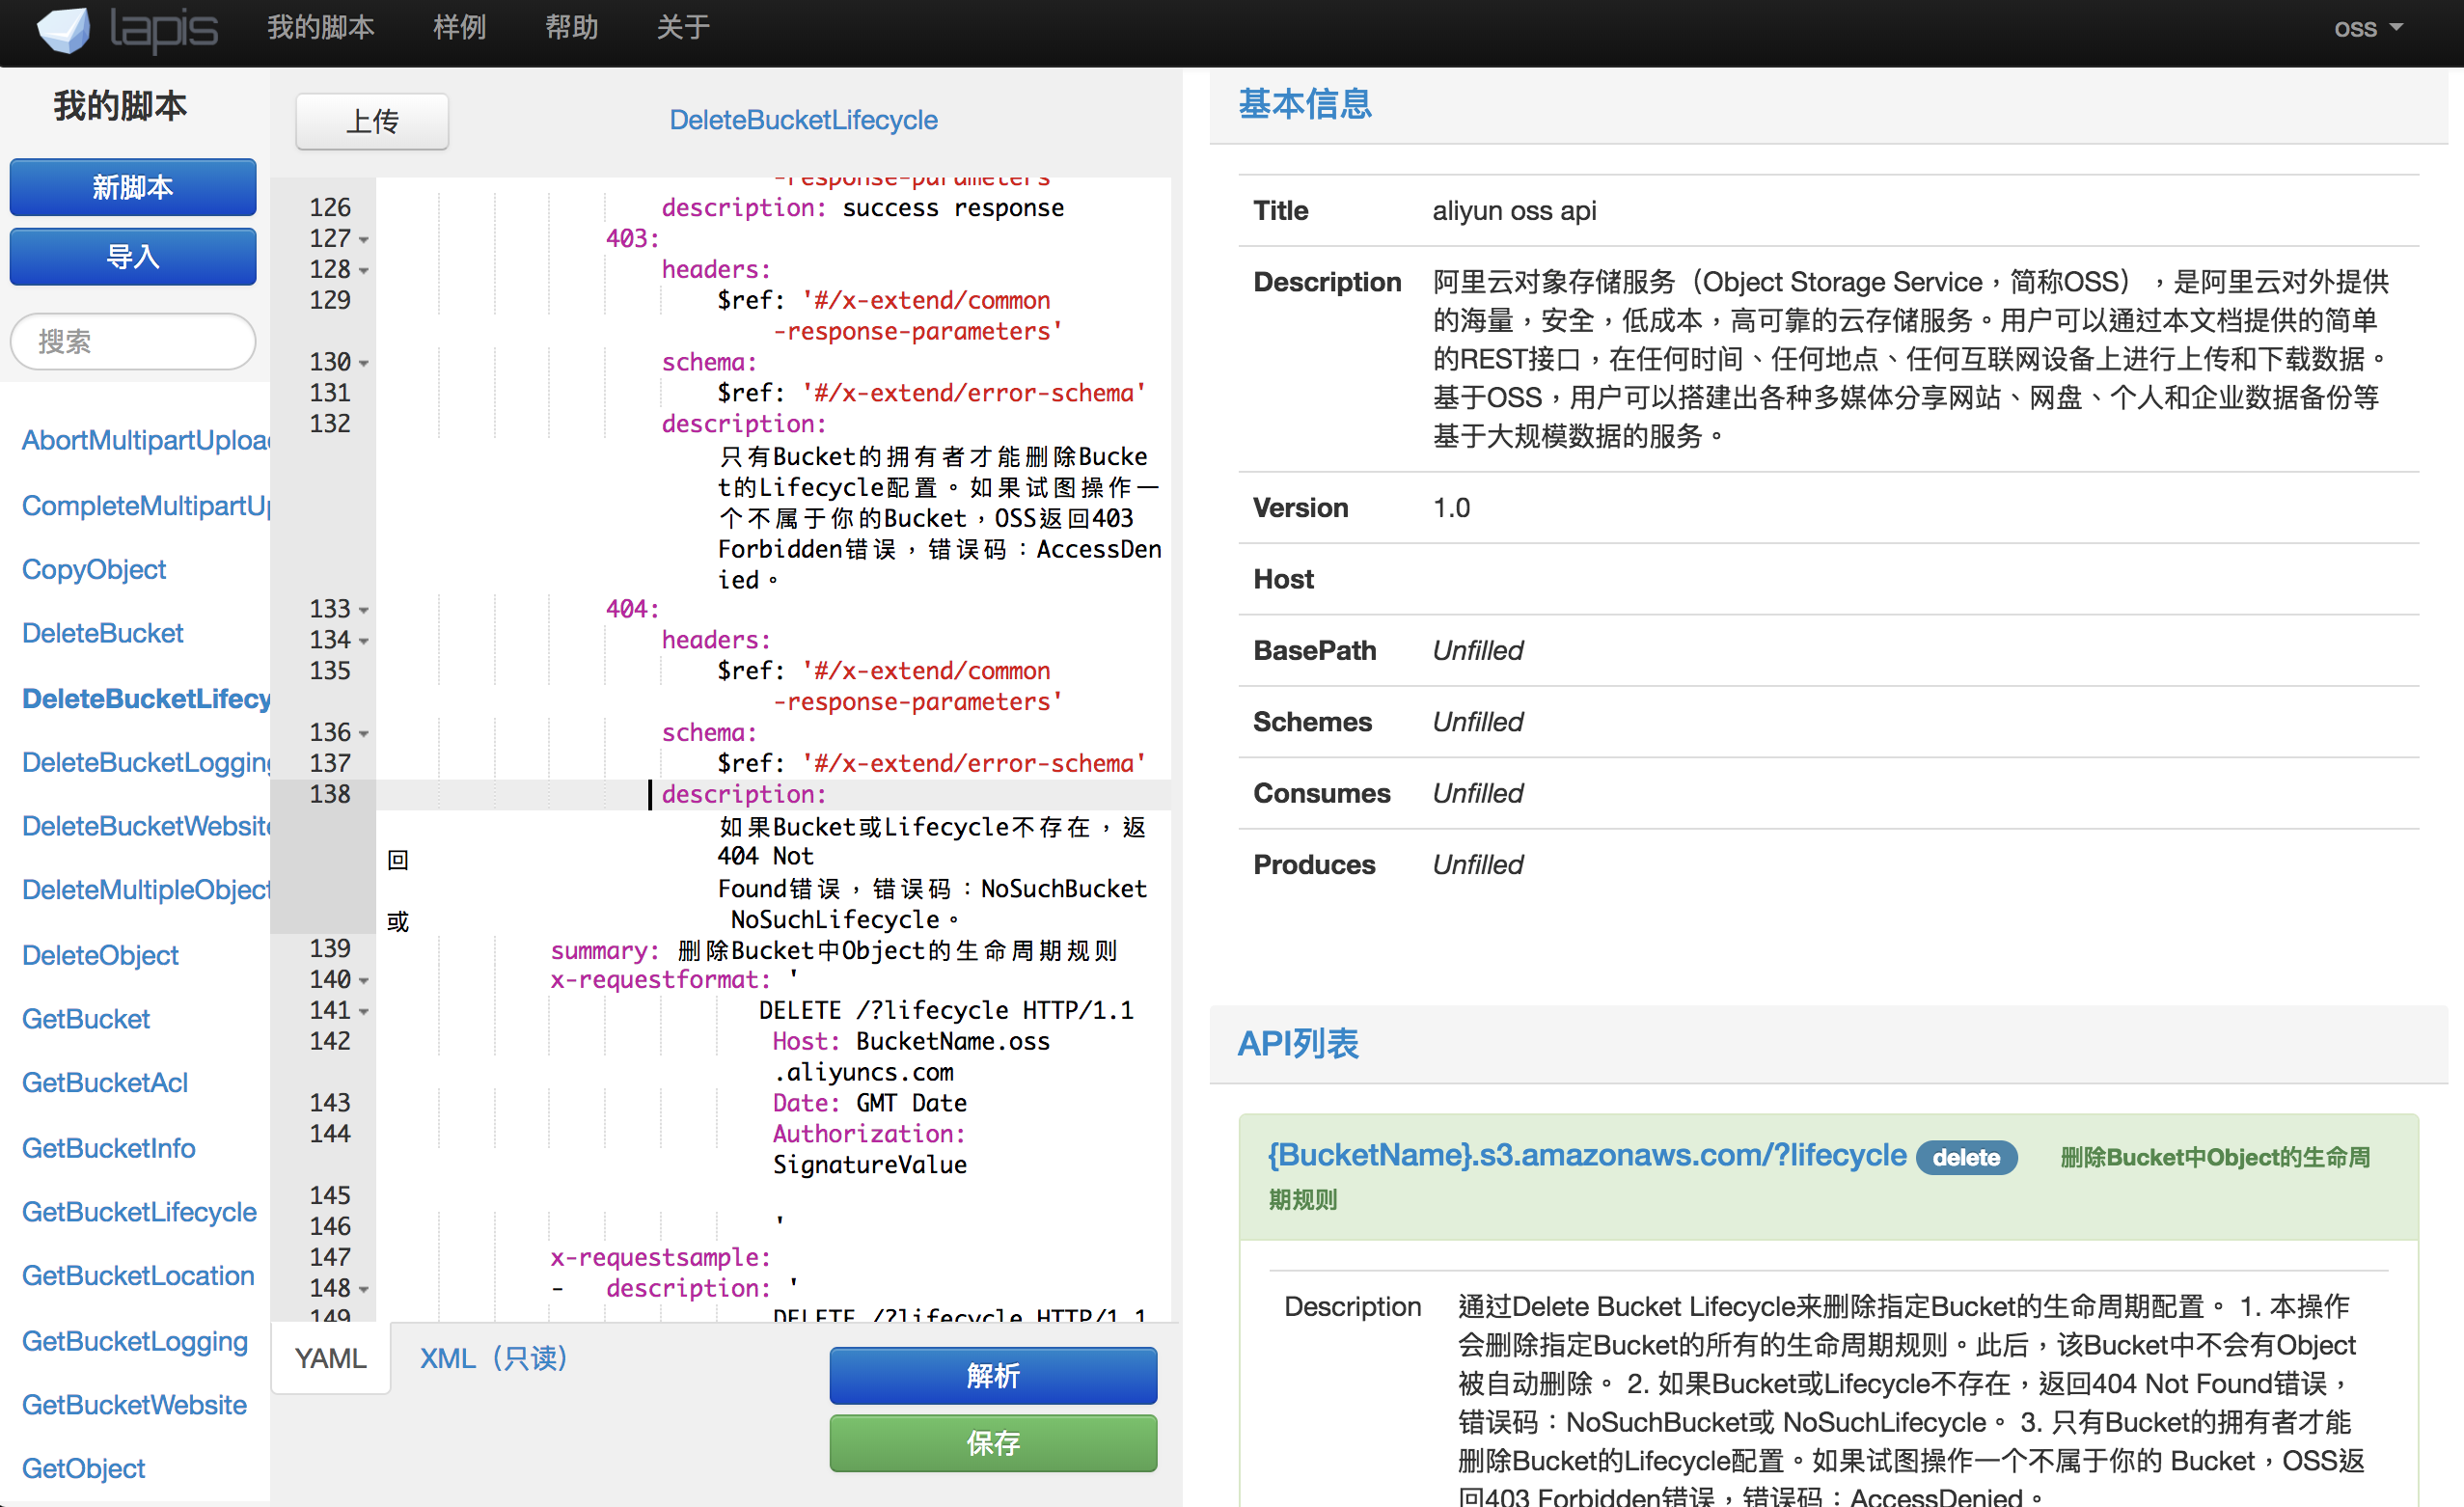
\includegraphics[width=200pt]{frontend_screenshot.png}
                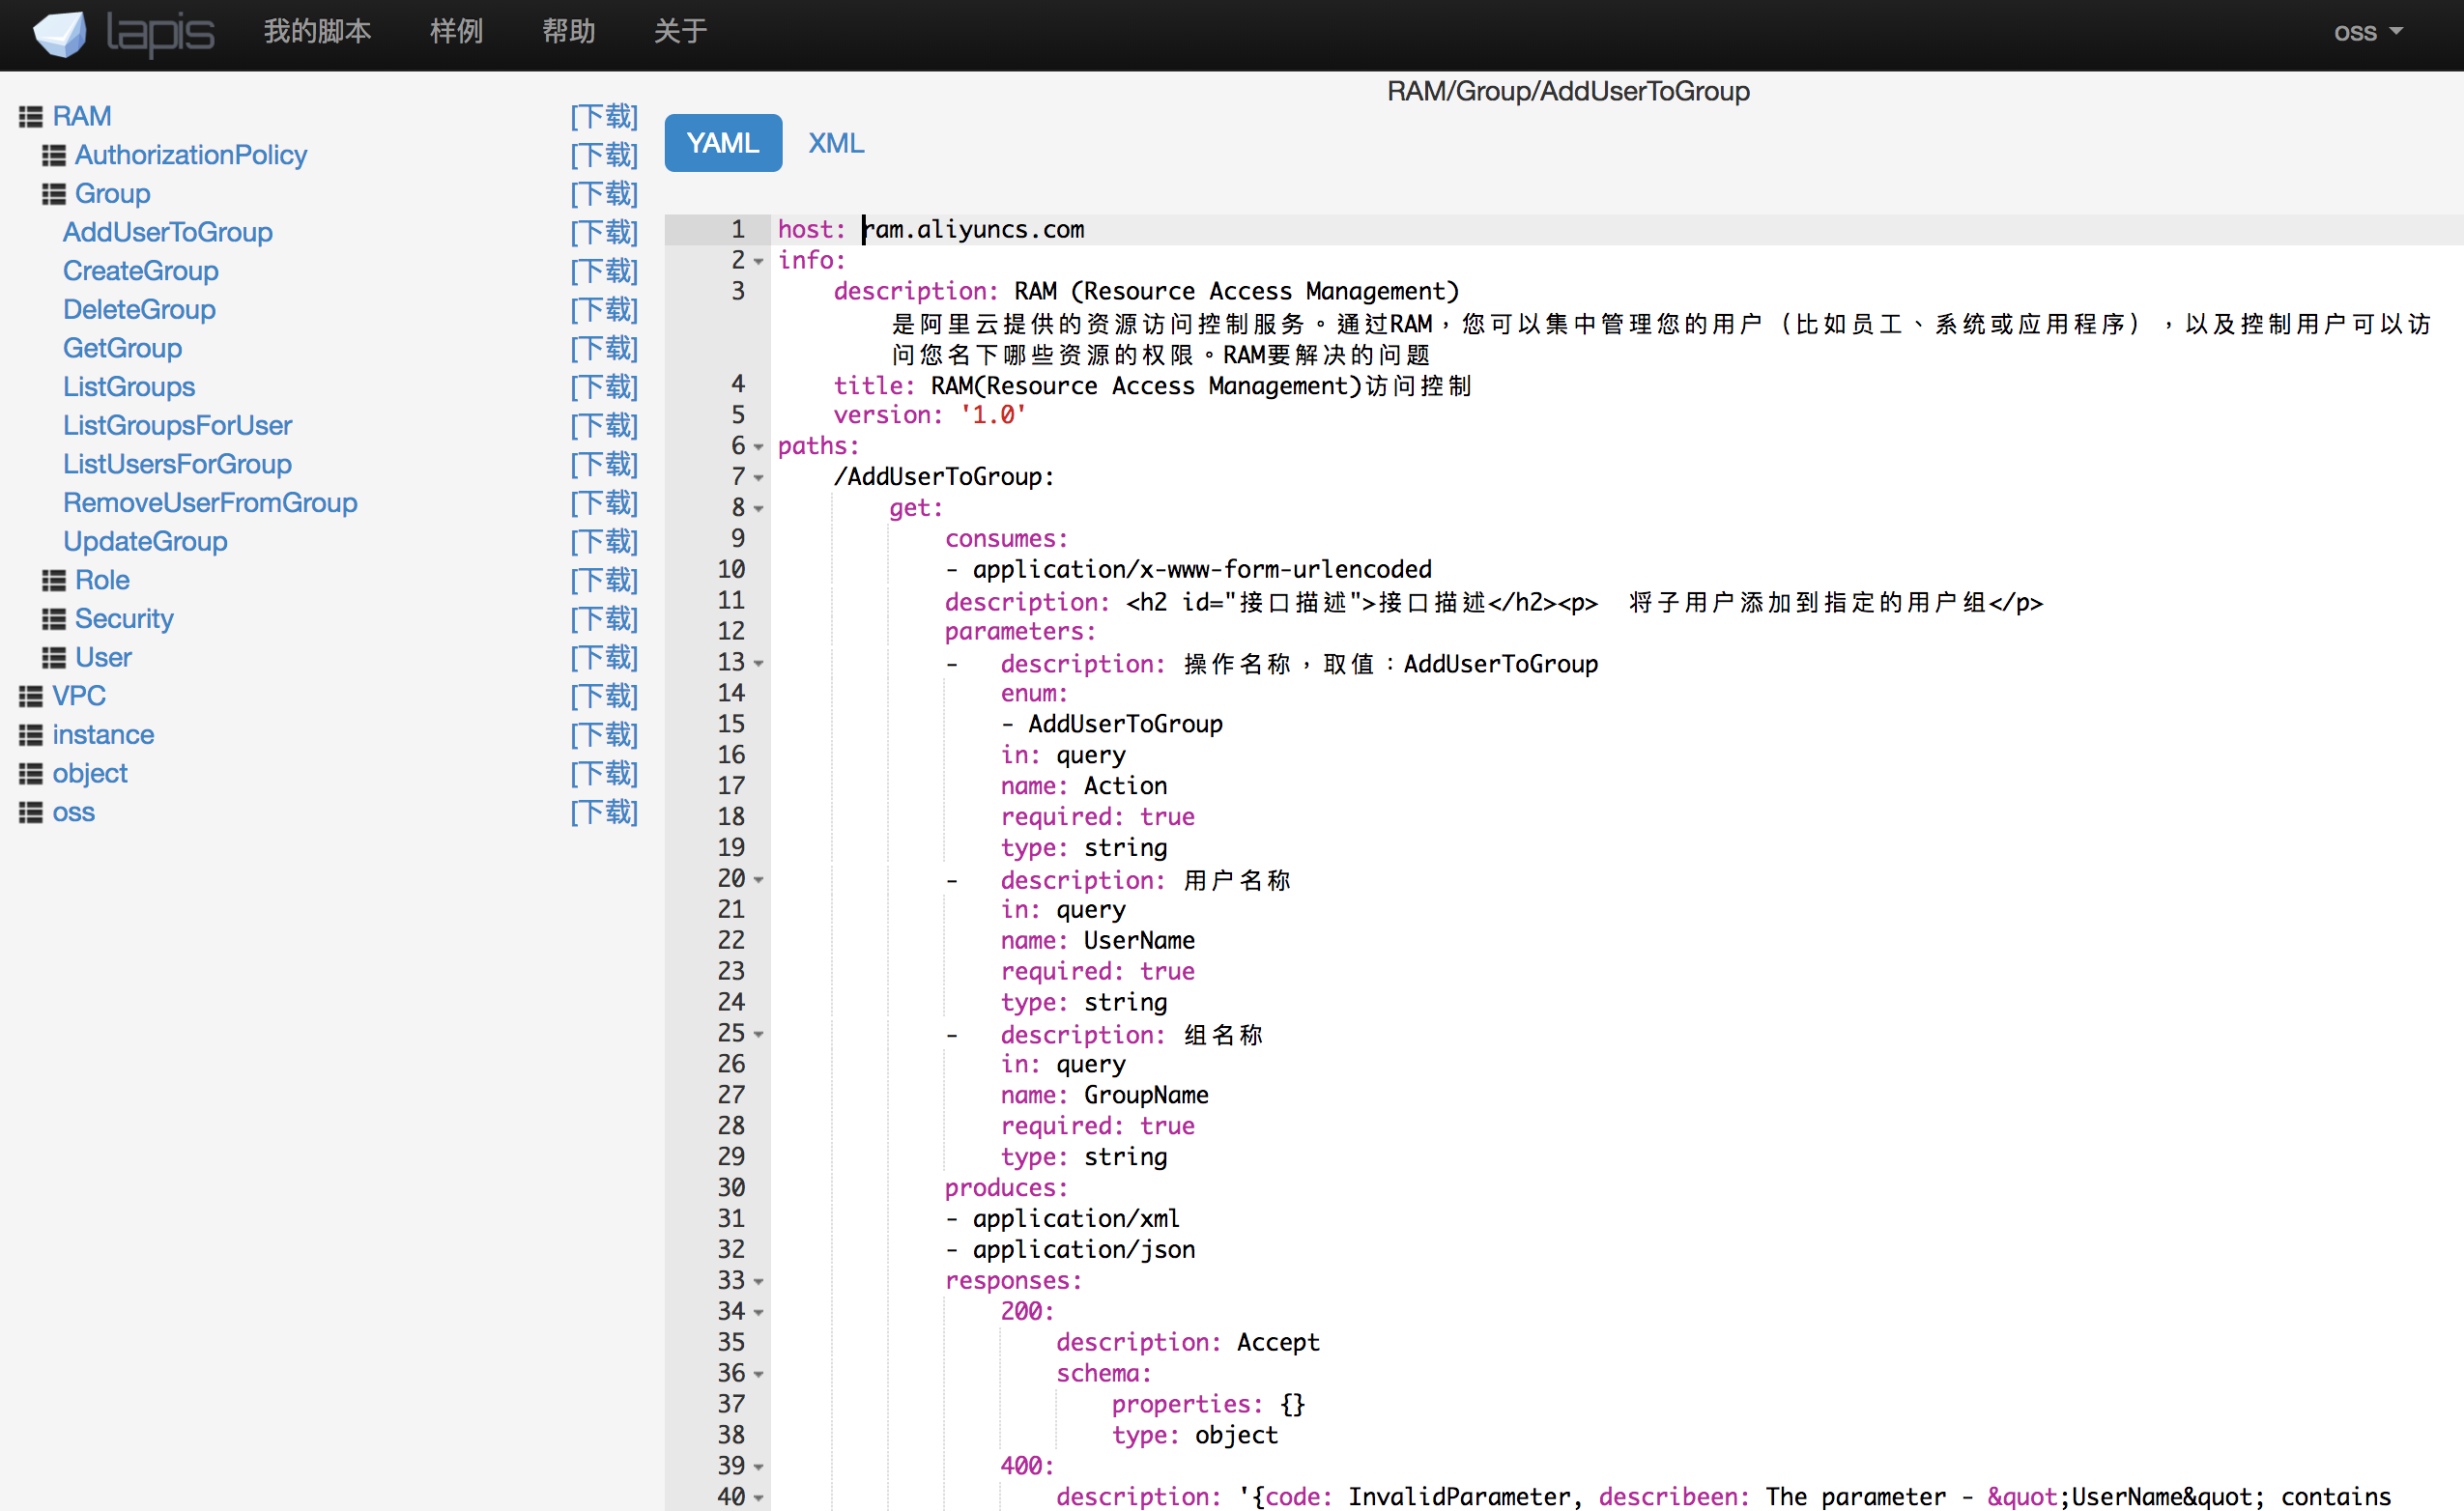
\includegraphics[width=200pt]{frontend_screenshot2.png}
                \caption{Web端脚本编辑系统前端截图. 通过此系统, 用户可以在线进行脚本的编辑与上传, 编辑时, 系统对API脚本进行实时解析, 以类似于API使用手册的形式展示脚本内容.}
                \label{fig:frontend_screenshot}
            \end{figure}
            
            本工作为API行为文档的编辑开发了一个在线web系统, 运行截图见图\ref{fig:frontend_screenshot}. 在此系统中, 用户可在线编辑与上传API行为文档, 并获得解析结果的实时反馈. 如果文档的内容合法, 前端会将所描述的API以类似于使用手册的形式进行可视化, 并展示于右栏. 为了提升可读性, 各个参数和响应体的展示采用折叠式的设计. 如果文档的内容不合法, 系统会提示出错原因与位置. 每个注册用户拥有私有文件夹, 后台记录了文件夹内各文档的历史版本, 文档也可从本地上传到此文件夹. 此外, 编辑系统还附带大量样例方便用户快速熟悉文档采用的OpenAPI规约语言.
            
            此web编辑系统的后端采用Python语言和Django框架, 前端采用JQuery和Bootstrap库. 直接依托文件系统实现了用户和文档托管功能, 无数据库依赖, 较轻量, 适合部署作为企业测试部门内部服务或单机使用.
        
            \label{sec:scenario_gui_edit}
            此外, 场景模型基于自动机模型, 故场景脚本一定程度上不适于采用直接编写的形式创建, 而适于用有向图表示, 并在图形化界面中拖拽绘制生成\cite{junyiw17}. 开发创建场景模型的图形化界面很可能将明显提高场景脚本的生成效率, 是未来可进一步研究的方向.
            
        % extended version
		% \subsection{*桌面端测试管理系统}


